\chapter{Introduction} \label{ch:introduction}
Quadrotor control is a difficult and interesting problem. A quadrotor has six degrees of freedom (three translational and three rotational) and four independent inputs (forces applied by the motors). As established by \cite{Liu2015} and \cite{Lopez2015}, quadrotor dynamics are affected by nonlinearity, parameters perturbations, uncertainties and disturbances: this include unknown and variable payloads, aerodynamical parameters of the system, wind changes, and sensors inaccuracies. Numerous studies have been developed in designing optimal and robust controllers that allow unmanned aircraft systems (UAS) to fly and accomplish missions rejecting disturbances and being robust to parameter uncertainties as seen in \cite{Jung2014, Kohno2014, Shang2016, Salazar2014}.\\\\
Although there are embedded systems with high computational capacity that can serve as controllers of a quadrotor, smartphones are available, easily accessible for people and also have a large computational capacity, hence multiple instrumentation and communication elements integrated in the same device. The use of smartphones also facilitates distribution and installation of updates of the control application as it is a commonly known device and has application distribution platforms. Some attempts to joint smartphones and aerial robots have been made: in \cite{Pearce2014a}, a smartphone was used as a mission planner for a quadrotor and in \cite{ALEMARK2014a}, a smartphone was used as flight controller using its sensors and power to stabilize the quadrotor and control its altitude. A smartphone has been used as a flight controller and processing system for image-based positioning in a quadrotor, as shown in \cite{Loianno2015}.
\\\\
This research project aims to design and implement algorithms that will be executed in a smartphone to estimate and control quadrotor dynamics by the Research Group in Industrial Control. This project confronts several challenges such as using a smartphone as a hardware development platform, trying to use a non real-time operating system for real-time applications, designing optimal and high order controllers using Java or C++, and executing that controllers in a smartphone.
\\\\
This paper presents the design of an optimal and a robust controller, and a state estimator based on a Kalman filter for a smartphone-based quadrotor. The non-linear and linerized model of the quadrotor is presented, the controller that allows the quadrotor to follow a trajectory reference using two approachs is designed. The two approaches are the LQG and $H_\infty$ controllers. The quadrotor flight dynamics estimation strategies using sensor fusion algorithms are described. 
\\\\
Current smartphone processors are able to perform complex calculations such as those required in the implementation of real time control strategies. There are many ongoing research related to the possibility of using smartphones to implement control strategies, such as \cite{Drumea2013a}, as configuration and monitoring interfaces in control systems as seen in \cite{Lin2014a,Truong2012a}, and as a tool in both education and design of control strategies seen in \cite{Aristizabal2014a,WuWu2013a}. Following this trend, in the Universidad del Valle, it was developed a smartphone-based platform for monitoring, control and communication in portable laboratories, where a controller for a pendulum based in the Lego Mindstorms EV3 platform was implemented \cite {GarciaTellez2015}.
\\\\
In recent years, the interest in aerial robotics research has increased substantially. This is because this type of robotics offers several potential new services such as search and rescue, observation, mapping, inspection, etc. On the other hand, smartphones have become essential devices for humans and easily acquirable development tools. The interaction between these two technologies allow the development of low cost quadcopters based on an everyday item such as the smartphones, facilitating the distribution of the quadcopter control software and its implementation by other researchers.
%~\ref{fig:quads500} for an example.
\begin{figure}[h]
\begin{center}
\includegraphics[width=8.6cm]{quadBasic1}    
\caption{Assembled quadcopter used in this research with the on-board smartphone on the top center of it.} 
\label{fig:quads500}
\end{center}
\end{figure}
\\\\
In the University of Pennsylvania, in \cite{Loianno2015}, was developed a quadcopter using a last generation smartphone as a flight controller and an additional processing system for image-based positioning. The state estimation algorithms, control and planning were firstly implemented in a ODROID-XU board with additional sensors, but then, in \cite{Loianno2015a}, this algorithms were ported to the Qualcomm processor in the phone due to the Qualcomm colaboration in that project.
\\\\
Current research focuses on the development of aerial robots potentiated by the use of smartphones, as seen in \cite{Pearce2014a, ALEMARK2014a, Aldrovandi2015, Bryant2015}. In the last years, computing capacity and sensor technology in smartphones has decreased in price but increased in performance. Smartphones have become an inexpensive tool capable of commanding an UAV. The challenge then, is to use smartphones as quadcopter flight controllers for autonomous flights following specific missions, taking advantage of the fact that the phones today are very powerful computers that include elements of sensing, processing and signal communication.
\\\\
In this paper, the implementation of a quadcopter with a smartphone acting as its flight controller while using exclusively the sensors and processor in the smartphone, is shown. The controller keeps the attitude of the quadcopter stabilized while making the quadcopter to hover at an altitude reference. It is presented the detailed composition of the test platform (quadcopter) used, integrating it with its dynamic model in addition to the quadcopter altitude and attitude estimation strategies using sensor fusion algorithms.
\section{Motivation}
wfwfew
\section{Research Problem}
En los últimos años el interés por la investigación en robótica aérea ha aumentado sustancialmente. Esto se debe a que este tipo de robótica ofrece diferentes servicios potenciales como búsqueda y rescate, observación, mapeo, inspección, entre otros. Por otro lado, los teléfonos inteligentes se han convertido en dispositivos esenciales para el ser humano y en herramientas de desarrollo y prototipado rápido de fácil acceso. La interacción entre estas dos tecnologías permitiría el desarrollo de cuadricópteros a bajo costo basados en un elemento cotidiano como los teléfonos inteligentes, facilitando la distribución del software de control y su implementación a manos de otros investigadores.
\\\\
Los  desafíos  de  investigación  existentes  están en  cómo  desarrollar  e  implementar  algoritmos eficientes de control para teléfonos inteligentes usando el sistema operativo Android, y  valorar,  adaptar  y  desarrollar  las  tecnologías  adecuadas  de  comunicación,  sensado  y actuación con los teléfonos inteligentes en la ejecución de misiones utilizando cuadricópteros.
\\\\
La pregunta a responder es ?`cómo desarrollar estrategias de control en un teléfono inteligente para el control de vuelo de un cuadricóptero de manera que se utilice la instrumentación y capacidad de computación del teléfono y se puedan desarrollar misiones utilizando un cuadricóptero?\\
\section{Objectives}
\subsubsection{Objetivo General}
Para responder a la pregunta de investigación se plantea el siguiente objetivo general:\\
Diseñar e implementar algoritmos de control y estimación de dinámicas de vuelo ejecutados en un teléfono inteligente para el cuadricóptero del Grupo de Investigación en Control Industrial.
\subsubsection{Objetivos Específicos}
\begin{enumerate}
\item Realizar un estudio y análisis del estado del arte relacionado con el control y la estimación de los estados de cuadricópteros.
\item Integrar el cuadricóptero existente con un telefono intelingente que contenga los sensores adecuados para el control y la estimación de estados.
\item Obtener un modelo dinámico del cuadricóptero.
\item Diseñar e implementar los algoritmos de control y de estimación de estados para el cuadricóptero.
\item Integrar la plataforma de experimentación con los algoritmos de control y estimación en el teléfono inteligente.
\item Evaluar el desempeño de las estrategias de control.%????
\end{enumerate}

\section{Literature Review}
wfwfewf

\subsection{Quadrotors}
wfwefwe


\subsection{Quadrotor Flight Modes}
\url{http://ardupilot.org/copter/docs/flight-modes.html}
\cite{Ardupilot2016}

\subsubsection{Stabilize Mode}
Stabilize mode allows you to fly your vehicle manually, but self-levels the roll and pitch axis.
\\\\
Pilot’s roll and pitch input control the lean angle of the copter. When the pilot releases the roll and pitch sticks the vehicle automatically levels itself.
    
    Pilot will need to regularly input roll and pitch commands to keep the vehicle in place as it is pushed around by the wind.
    
    Pilot’s yaw input controls the rate of change of the heading. When the pilot releases the yaw stick the vehicle will maintain it’s current heading.
    
    Pilot’s throttle input controls the average motor speed meaning that constant adjustment of the throttle is required to maintain altitude. If the pilot puts the throttle completely down the motors will go to their minimum rate (MOTSPINARMED) and if the vehicle is flying it will lose attitude control and tumble.
    
    The throttle sent to the motors is automatically adjusted based on the tilt angle of the vehicle (i.e. increased as the vehicle tilts over more) to reduce the compensation the pilot must do as the vehicle’s attitude changes.

\subsubsection{Altitude Hold Mode}
In altitude hold mode, Copter maintains a consistent altitude while allowing roll, pitch, and yaw to be controlled normally. This page contains important information about using and tuning alt hold.
\\\\
When altitude hold mode (aka AltHold) is selected, the throttle is automatically controlled to maintain the current altitude. Roll, Pitch and yaw operate the same as in Stabilize mode meaning that the pilot directly controls the roll and pitch lean angles and the heading.
\\\\
Automatic altitude hold is a feature of many other flight modes (Loiter, Sport, etc) so the information here pertains to those modes as well.
\\\\
The pilot can control the climb or descent rate of the vehicle with the throttle stick.

    If the throttle stick is in the middle (40$\%$ ~ 60$\%$) the vehicle will maintain the current altitude.
    Outside of the mid-throttle deadzone (i.e. below 40$\%$ or above 60$\%$) the vehicle will descend or climb depending upon the deflection of the stick. When the stick is completely down the copter will descend at 2.5m/s and if at the very top it will climb by 2.5m/s.

\subsubsection{Loiter Mode}
Loiter Mode automatically attempts to maintain the current location, heading and altitude. The pilot may fly the copter in Loiter mode as if it were in a more manual flight mode but when the sticks are released, the vehicle will slow to a stop and hold position.
\\\\
A good GPS lock, low magnetic interference on the compass and low vibrations are all important in achieving good loiter performance.
\\\\
The pilot can control the copter’s position with the control sticks.

    Horizontal location can be adjusted with the the Roll and Pitch control sticks with the default maximum horizontal speed being 5m/s (see Tuning section below on how to adjust this). When the pilot releases the sticks the copter will slow to a stop.
    Altitude can be controlled with the Throttle control stick just as in AltHold mode
    The heading can be set with the Yaw control stick

\subsubsection{Return-To-Launch Mode}
When RTL mode is selected, the copter will return to the home location. The copter will first rise to RTLALT before returning home or maintain the current altitude if the current altitude is higher than RTLALT. The default value for RTLALT is 15m.
\\\\
RTL is a GPS-dependent move, so it is essential that GPS lock is acquired before attempting to use this mode. Before arming, ensure that the APM’s blue LED is solid and not blinking. For a GPS without compass, the LED will be solid blue when GPS lock is acquired. For the GPS+Compass module, the LED will be blinking blue when GPS is locked.
\\\\
RTL will command the copter to return to the home position, meaning that it will return to the location where it was armed. Therefore, the home position is always supposed to be your copter’s actual GPS takeoff location, unobstructed and away from people. For Copter if you get GPS lock and then ARM your copter, the home position is the location the copter was in when it was armed. This means if you execute an RTL in Copter, it will return to the location where it was armed.

\subsubsection{Auto Mode}
In Auto mode the copter will follow a pre-programmed mission script stored in the autopilot which is made up of navigation commands (i.e. waypoints) and “do” commands (i.e. commands that do not affect the location of the copter including triggering a camera shutter). This page provides an overview of Auto mode.


\subsection{Smartphones as Controllers}
wfwfwewf

\subsection{Smartphone-based Quadrotors}
wfwfwf

\subsubsection{Smartphone-based Quadrotor Limitations}
The idea of using a smartphone as flight controller in an UAV opens the possibility of a rapid and inexpensive development \cite{Aldrovandi2015}. A smartphone offers other advantages compared with off-the-shelf flight controllers, for instance its powerful quad or hexa-core processors and communications interfaces. However, smartphones and the Android operating system have some limitations that set challenges when implementing a control system in it.\\\\
Android is not a real-time operating system and thus can not assure execution of algorithms, like estimation and control, with a constant sample time. Furthermore, the sensors embedded in commercial smartphones are made for applications that do not have high requirements of accuracy nor precision and therefore may not be appropriate for sensing quadrotor dynamics. Nonetheless, as explained by \cite{Bryant2015}, due to its computing capabilities, smartphones can overcome this limitations while using a temporized thread to execute the control system algorithms and implement a sensor fusion technique to improve the states estimation reliability. This thread must be executed with a lower sample time compared to the one of the sensors embedded in the smartphone. This will ensure that the execution is not delayed by the sensors acquisition process.

\section{Outline}
In the next section, a detailed description of the hardware used in the quadcopter is presented. After that, the dynamic non-linear and linearized quadcopter model is shown in Section \ref{sec:Model}. In Section \ref{sec:Controller}, all the aspects related to the altitude and attitude cascade controllers design are presented.
Then, in Section \ref{sec:Estimation} the sensor fusion algorithm that is used to estimate the altitude of the quadcopter, and how the orientation of the system is estimated, is described. In Section \ref{sec:Implementation}, the implementation in Android of all the necessary software with its results is provided. Finally, Section \ref{sec:Conclusion} concludes this paper taking into account the results of this research and the future work to be done.
\\\\
This paper is organized as follows: The smartphone-based quadrotors features and limitations are shown in Section \ref{sec:limitations}. In Section \ref{sec:Model}, the dynamic model of a quadrotor in $X$-configuration using a Newton-Euler approach is presented. After that, in Section \ref{sec:controllers}, the quadrotor parameters and controllers design procedure is exposed. In Section \ref{sec:estimation}, the state estimation algorithms based on a Kalman filter and the kinematic model of a particle with constant acceleration are provided. The performance of the proposed flight control system through simulations is presented in Section \ref{sec:simulation}. Finally, Section \ref{sec:conclusions} shows the conclusions and future aiming of this project.

%\section{Multi-Agent Systems}
%
%
%Advances in exploration and rescue technologies become more relevant than ever before.
%
%In an effort to develop distributed mobile agent systems able to resemble their natural counterparts, engineers have been experimenting with mobile sensor networks trying, for example, to implement flocking applications.  The goal has been to create self-organized networks  capable of coordinated group behaviour \citep{MateiBaras12}. For this purpose, heuristic rules were introduced by \citep{SpanosOlfatiMurray05} in order to explain any form of collective behaviour of a large number of individuals  with a common goal. These rules are known as cohesion, separation, and alignment. Cohesion means the attempt to stay close to  the neighbours, separation means avoiding collisions with neighbours, and alignment means the attempt to match velocity with neighbour agents. 
%
%
% For example, oil spilled in the sea generates a scalar field of oil concentration values (Fig. \ref{fig:oilspill}). Similarly,  radiation levels after  nuclear disaster like in Fukushima (Fig.  \ref{fig:fukushima_1}), or a toxic substance cloud moving in space are  phenomena that can be represented as scalar fields (Fig. \ref{fig:scalarfieldsource}). 
%\afterpage{
%\begin{figure}[ht!]
%        \centering
%        \begin{subfigure}[t]{0.49\textwidth}
%                \includegraphics[width=\textwidth]{oilspill.eps}
%                \caption{Oil spill \footnotemark} 
%                \label{fig:oilspill}
%        \end{subfigure}%
%        ~ %add desired spacing between images, e. g. ~, \quad, \qquad etc.
%          %(or a blank line to force the subfigure onto a new line)
%        \begin{subfigure}[t]{0.49\textwidth}
%                \includegraphics[width=\textwidth]{fukushima_1.eps}
%                \caption{Fukushima's environment radiation levels after nuclear disaster  \footnotemark}
%                \label{fig:fukushima_1}
%        \end{subfigure}
%        ~ %add desired spacing between images, e. g. ~, \quad, \qquad etc.
%          %(or a blank line to force the subfigure onto a new line)
%        \begin{subfigure}[t]{0.62\textwidth}
%                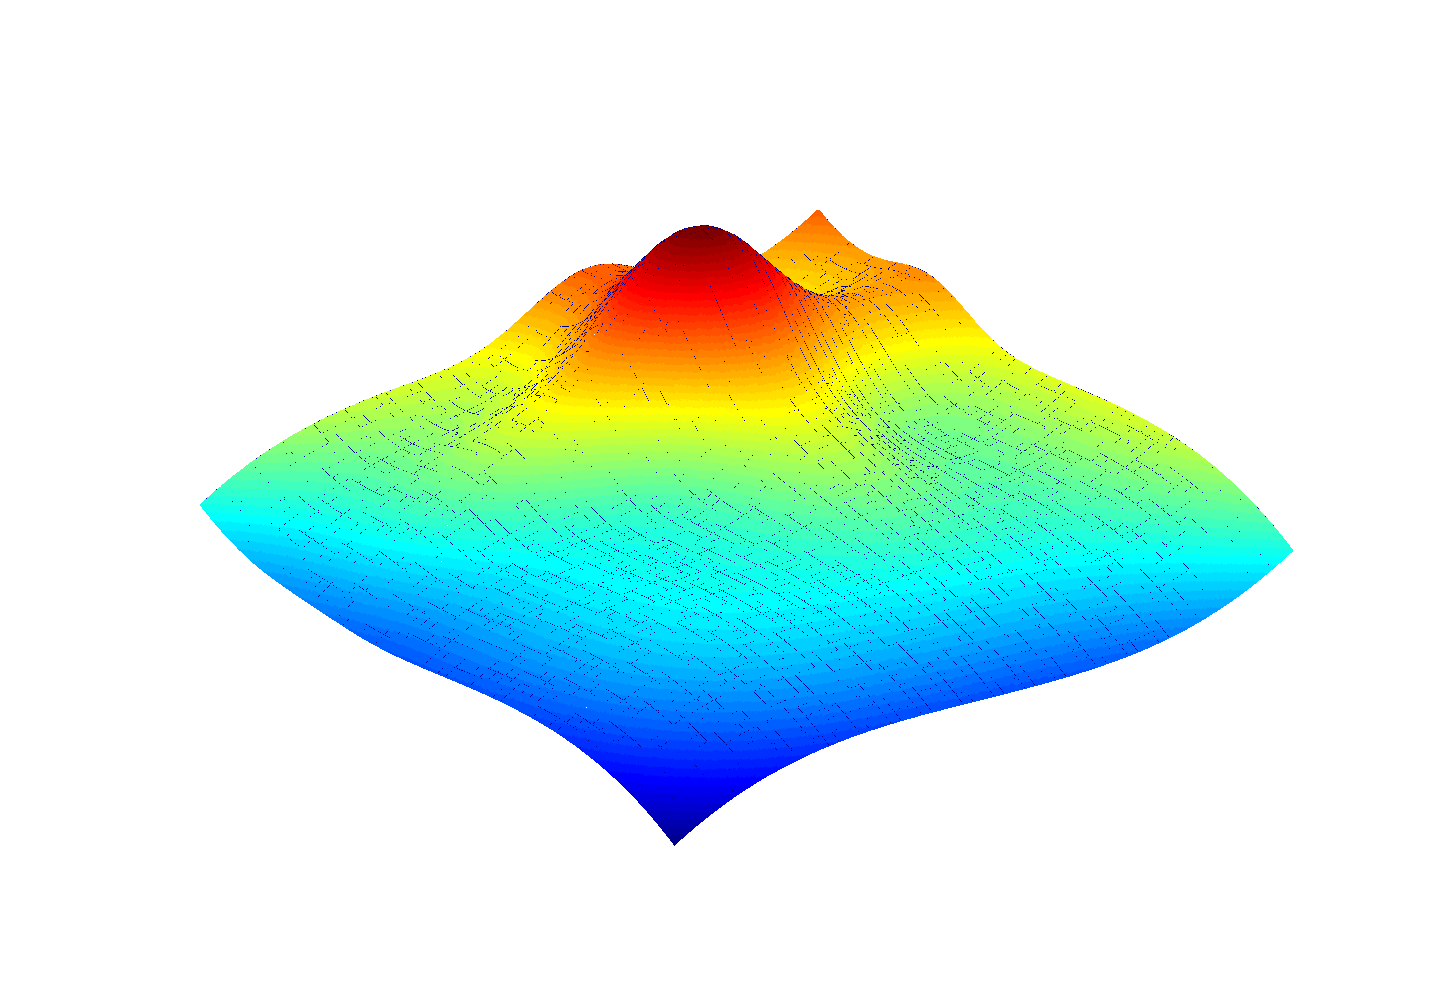
\includegraphics[width=\textwidth]{scalarfieldsource.eps}
%                \caption{Toxic cloud}
%                \label{fig:scalarfieldsource}
%        \end{subfigure}%
%        ~ %add desired spacing between images, e. g. ~, \quad, \qquad etc.
%          %(or a blank line to force the subfigure onto a new line)
%       \caption{Scalar fields} \label{fig:scalar field}
%\end{figure}
%\footnotetext[1]{Picture taken from FeedNetBack project}
%\footnotetext[2]{Picture taken from seaandskyjp.wordpress.com}
%}
% 


